\documentclass[11pt]{article}

\usepackage[letterpaper,margin=0.75in]{geometry}
\usepackage{booktabs}
\usepackage{graphicx}
\usepackage{listings}
\usepackage{mathtools}

\setlength{\parindent}{1.4em}

\begin{document}

\lstset{
  language=Python,
  basicstyle=\small,          % print whole listing small
  keywordstyle=\bfseries,
  identifierstyle=,           % nothing happens
  commentstyle=,              % white comments
  stringstyle=\ttfamily,      % typewriter type for strings
  showstringspaces=false,     % no special string spaces
  numbers=left,
  numberstyle=\tiny,
  numbersep=5pt,
  frame=tb,
}

\title{Lab 1 Report}

\author{Dallin Christensen}

\date{January 24, 2014}

\maketitle

\section{Two Nodes}

To simulate a two node network, I created two nodes (n1 and n2) linked together by a bidirectional link. I defined a setup function that would create the network with passed in values for bandwidth and propagation delay, returning the two nodes of the network.
\vspace{0.5cm}

\begin{lstlisting}
def TwoNodeSetup(b, p):
    Sim.scheduler.reset()

    # setup network
    n1 = node.Node()
    n2 = node.Node()

    l = link.Link(address=1, startpoint=n1, endpoint=n2, bandwidth=b, propagation=p)
    n1.add_link(l)
    n1.add_forwarding_entry(address=2, link=l)
    
    l = link.Link(address=2, startpoint=n2, endpoint=n1, bandwidth=b, propagation=p)
    n2.add_link(l)
    n2.add_forwarding_entry(address=1, link=l)
    
    d = DelayHandler()
    n2.add_protocol(protocol="delay", handler=d)

    return n1, n2
\end{lstlisting}

\begin{enumerate}
\item Scenario 1 \hfill \\
The first scenario was a network with a link bandwidth of 1 Mbps and a propagation delay of 1 second. One packet of 1000 bytes was created at time 0, sent from n1 immediately, and received by n2 at time 1.008 seconds.

\begin{description}
\item[Calculation] \hfill \\
$$Transmission Delay = \frac{L}{R} = \frac{1,000 bytes}{1 Mbps} = \frac{8,000 bits}{1,000,000 bps}$$
$$Propagation Delay = 1 second$$
$$TotalTime = \frac{8,000 bits}{1,000,000 bps} + 1 second = 0.008 + 1 = 1.008 seconds$$

This result is consistent with the output given by the simulator.
\end{description}

\item Scenario 2 \hfill \\
The second scenario was a network with a link bandwidth of 100 bps and a propagation delay of 10 ms. One packet of 1000 bytes was created at time 0, sent from n1 immediately, and received by n2 at time 80.01 seconds.

\begin{description}
\item[Calculation] \hfill \\
$$Transmission Delay = \frac{L}{R} = \frac{1,000 bytes}{100 bps} = \frac{8,000 bits}{100 bps}$$
$$Propagation Delay = 10 ms = 0.01 seconds$$
$$TotalTime = \frac{8,000 bits}{100 bps} + 0.01 seconds = 80 + 0.01 = 80.01 seconds$$

This result is consistent with the output given by the simulator.
\end{description}

\item Scenario 3 \hfill \\
The third scenario was a network with a link bandwidth of 1 Mbps and a propagation delay of 10 ms. Three packets of 1000 bytes apiece were created at time 0 and sent from n1 immediately. A fourth packet of 1000 bytes was created at time 2 seconds and sent from n1 immediately. The packets were received by n2 at times 0.018 seconds, 0.026 seconds, 0.034 seconds, and 2.018 seconds, respectively.

\begin{description}
\item[Calculation] \hfill \\
$$Transmission Delay = \frac{L}{R} = \frac{1,000 bytes}{1 Mbps} = \frac{8,000 bits}{1,000,000 bps}$$
$$Propagation Delay = 10 ms = 0.01 seconds$$
$$FirstPacketTime = \frac{8,000 bits}{1,000,000 bps} + 0.01 seconds = 0.008 + 0.01 = 0.018 seconds$$
$$SecondPacketTime = \frac{8,000 bits}{1,000,000 bps}*2 + 0.01 seconds = 0.016 + 0.01 = 0.026 seconds$$
$$ThirdPacketTime = \frac{8,000 bits}{1,000,000 bps}*3 + 0.01 seconds = 0.024 + 0.01 = 0.034 seconds$$
$$FourthPacketTime = 2 seconds + \frac{8,000 bits}{1,000,000 bps} + 0.01 seconds = 2 + 0.0008 + 0.01 = 2.018 seconds$$

These results are consistent with the output given by the simulator.
\end{description}

\end{enumerate}

\section{Three Nodes}

To simulate a three node network, I created three nodes (n1, n2, and n3) linked together by two bidirectional links (n1-n2, n2-n3). I defined a setup function that would create the network with passed in values for bandwidth and propagation delay for each link, returning the three nodes of the network.

\vspace{0.5cm}
\begin{lstlisting}
def ThreeNodeSetup(b1, b2, p1, p2):
    Sim.scheduler.reset()

    # setup network
    n1 = node.Node()
    n2 = node.Node()
    n3 = node.Node()
    
    l = link.Link(address=1, startpoint=n1, endpoint=n2, bandwidth=b1, propagation=p1)
    n1.add_link(l)
    n1.add_forwarding_entry(address=2, link=l)
    
    l = link.Link(address=2, startpoint=n2, endpoint=n1, bandwidth=b1, propagation=p1)
    n2.add_link(l)
    n2.add_forwarding_entry(address=1, link=l)

    l = link.Link(address=3, startpoint=n2, endpoint=n3, bandwidth=b2, propagation=p2)
    n2.add_link(l)
    n2.add_forwarding_entry(address=4, link=l)
    
    l = link.Link(address=4, startpoint=n3, endpoint=n2, bandwidth=b2, propagation=p2)
    n3.add_link(l)
    n3.add_forwarding_entry(address=3, link=l)

    d = DelayHandler()
    n3.add_protocol(protocol="delay", handler=d)

    return n1, n2, n3
\end{lstlisting}

\begin{enumerate}
\item Scenario 1 \hfill \\
The first scenario was a network with two fast links. Both links had a bandwidth of 1 Mbps and a propagation delay of 100 ms. 1000 packets of 1000 bytes (thus totaling 1 MB) were created at time 0 and put in n1's queue with n3 as their final destination.
\begin{center}
\begin{tabular}{ c c c c c c c }
  \multicolumn{7}{c}{Simulator Output} \\
  \hline
  {\tiny Total Time} & {\tiny Packets Sent} & {\tiny Start Time} & {\tiny End Time - Start Time} & {\tiny Transmission Delay} & {\tiny Propagation Delay} & {\tiny Queueing Delay}\\
  8.1 & 1000 & 0 & 8.1 & 0.008 & 0.1 & 7.992 \\
\end{tabular}
\end{center}
The simulator output is correct because
$$Total Time$$
$$= (numberOfPackets * transmissionDelay) + propagationDelay$$
$$= (1000*0.008) + 0.1 = 8.1 seconds$$
The total queueing delay is high because we added all of the packets to n1 at time 0.

\begin{enumerate}
    \item If both links are upgraded to a rate of 1 Gbps, how long does it take to transfer a 1 MB file from A to C?
    \begin{center}
    \begin{tabular}{ c c c c c c c }
      \multicolumn{7}{c}{Simulator Output} \\
      \hline
      {\tiny Total Time} & {\tiny Packets Sent} & {\tiny Start Time} & {\tiny End Time - Start Time} & {\tiny Transmission Delay} & {\tiny Propagation Delay} & {\tiny Queueing Delay}\\
      0.108 & 1000 & 0 & 0.108 & 0.000008 & 0.1 & 0.007992 \\
    \end{tabular}
    \end{center}
    The simulator output is correct because
    $$Total Time$$
    $$= (numberOfPackets * transmissionDelay) + propagationDelay$$
    $$= (1000*0.000008) + 0.1 = 0.0108 seconds$$
\end{enumerate}

\item Scenario 2 \hfill \\
The second scenario was a network with one fast link and one slow link. The fast link (between n1 and n2) had a bandwidth of 1 Mbps and a propagation delay of 100 ms, while the slow link (between n2 and n3) had a bandwidth of 256 Kbps and a propagation delay of 100 ms. 1000 packets of 1000 bytes (thus totaling 1 MB) were created at time 0 and put in n1's queue with n3 as their final destination.
\begin{center}
\begin{tabular}{ c c c c c c c }
  \multicolumn{7}{c}{Simulator Output} \\
  \hline
  {\tiny Total Time} & {\tiny Packets Sent} & {\tiny Start Time} & {\tiny End Time - Start Time} & {\tiny Transmission Delay} & {\tiny Propagation Delay} & {\tiny Queueing Delay}\\
  31.35 & 1000 & 0 & 31.35 & 0.03125 & 0.1 & 31.21875 \\
\end{tabular}
\end{center}
The simulator output is correct because
$$Total Time$$
$$= (numberOfPackets * transmissionDelay) + propagationDelay$$
$$= (1000*0.03125) + 0.1 = 31.35 seconds$$

\end{enumerate}

\section{Queueing Theory}

To set up the queueing delay simulation, I used the provided delay.py code with a slight modification. I would define a load (as a percentage), then output the queueing delay for each packet to a text file named after the load percentage.

\vspace{0.5cm}
\begin{lstlisting}
class DelayHandler(object):
    def define_load(self, load_percent):
        self.load_percent = load_percent
    def handle_packet(self,packet):
        # print Sim.scheduler.current_time(),packet.ident,packet.created,Sim.scheduler.current_time() - packet.created,packet.transmission_delay,packet.propagation_delay,packet.queueing_delay
        filename = "./delay_output/%s.txt" % self.load_percent
        with open(filename, "a") as filetowrite:
            filetowrite.write(str(packet.queueing_delay)+"\n")

if __name__ == '__main__':
    # parameters
    Sim.scheduler.reset()
    
    # setup packet generator
    max_rate = 1000000/(1000*8)
    load_percent = 0.98
    load = load_percent*max_rate

    # setup network
    n1 = node.Node()
    n2 = node.Node()
    l = link.Link(address=1,startpoint=n1,endpoint=n2)
    n1.add_link(l)
    n1.add_forwarding_entry(address=2,link=l)
    l = link.Link(address=2,startpoint=n2,endpoint=n1)
    n2.add_link(l)
    n2.add_forwarding_entry(address=1,link=l)
    d = DelayHandler()
    d.define_load(load_percent)
    n2.add_protocol(protocol="delay",handler=d)

    # packet generator
    g = Generator(node=n1, load=load,duration=10)
    Sim.scheduler.add(delay=0, event='generate', handler=g.handle)
    
    # run the simulation
    Sim.scheduler.run()
\end{lstlisting}
\vspace{0.5cm}

Using the queueing delay data stored in the text files, I plotted the results against the theoretical curve. 

\begin{center}
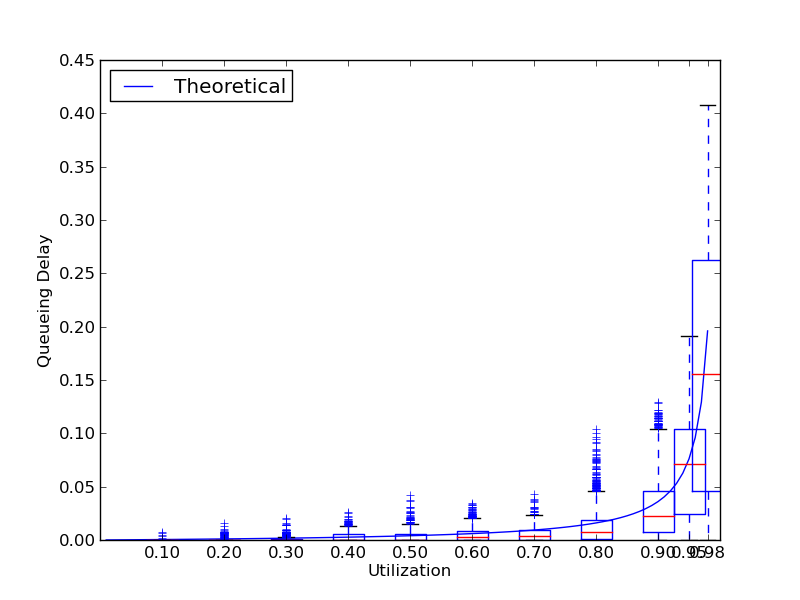
\includegraphics[width=11cm]{../bar}
\end{center}
\begin{center}
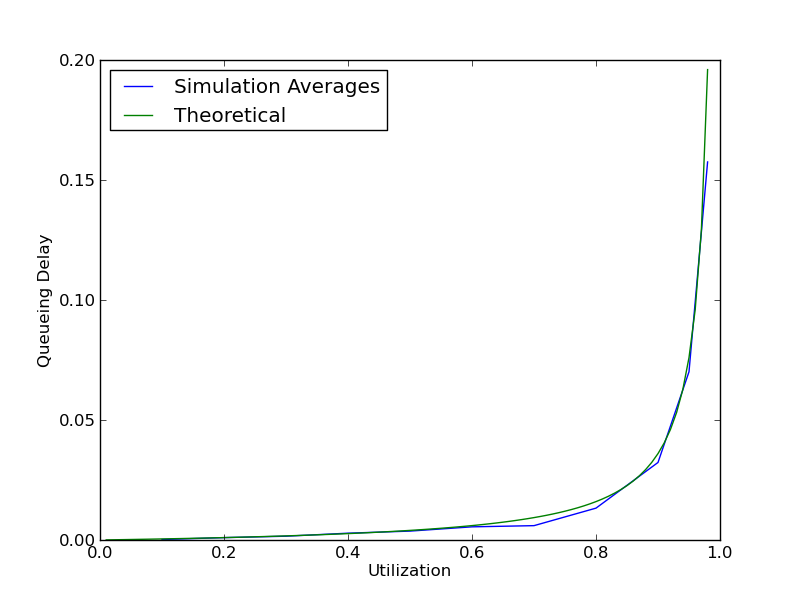
\includegraphics[width=11cm]{../average}
\end{center}

The simulator follows the theoritical curve nearly perfectly, which is to be expected from a simulator.
\end{document}
